\documentclass{article}
\usepackage[utf8]{inputenc}

\title{Implementing Wavelet Transforms on Many-core Architectures ---
        Using CUDA}
\author{Samuel Li}
\date{May 2015}

\usepackage{natbib}
\usepackage{graphicx}
\usepackage{color}
\newcommand{\fix}[1]{\textcolor{red}{#1}} %Put words in Red

\begin{document}

\maketitle

% \begin{abstract}
% \end{abstract}

\section{Introduction}
\label{sec:intro}
%
Wavelet transform is a technique rooted from the signal processing 
community~\cite{daubechies1990wavelet, mallat1999wavelet},
and soon people discovered its capacity in data reduction.
%
One of the most prominent uses of wavelet in data reduction has been
the JPEG2000 still image compression
standard~\cite{adams2001jpeg,usevitch2001tutorial}. 

In the scientific simulation and visualization field, researchers have
explored the use of discrete wavelet transforms (DWT) in two 
relative different directions, both aiming data reduction.
%
In the first direction, researchers use the DWT to provide data access
in a multi-resolution fashion, meaning that an approximation of the volume data
set is loaded at a lower resolution at first, and the particular region of interest
is then reconstructed with higher resolutions~\cite{mallat1989theory,
kanai1998digital, baldwin2003multi}.
%
In the second direction, the volume data is reconstructed at the 
original resolution, but using a subset of the wavelet transformed 
data.
%
The second direction results in a lossy compression~\cite{bethel2012high,
norton2012vapor}.

In a typical use case, the DWT is normally applied on each dimension of a
volume data set (e.g. X, Y, and Z dimension). 
%
Moreover, in practice, people always apply multiple rounds of DWT to achieve better
data reduction. 
%
The overall DWT on a volume data set is then becoming a heavy computation
task in most systems.
%
As a result, people need a faster way to calculate DWT. 

Many-core architectures have emerged recently as accelerators for a 
traditional computer system.
%
On the one hand, these accelerator cards have much more compute units 
than a traditional CPU (some NVidia GPUs have thousands of compute units).
%
On the other hand, the compute units on these accelerator cards are 
relatively simple compared to a CPU, making them not suitable for complex 
computational tasks.

DWT requires repetitive calculation on arrays of data, with little to no
dependency between different arrays.
%
The actual calculations performed on data items are convolutions
with the given filters. 
%
The width of the wavelet filter decides how many data items are 
involved in one convolution, which is usually no more than ten.
%
To parallelize this calculation, many convolutions can be performed
at the same time.
%
From the perspective of parallel computing, this process is applying
a stencil pattern.
%
%Such problems would perfectly fit into the many-core architecture, once we
%successfully implemented the DWT calculation of a single array on a 
%target many-core architecture.
%
In this term project, I am going to explore parallelizing the DWT algorithm 
to fit into the many-core architectures.


\section{Implementation Plan}
\label{sec:plan}
%
Update: 
%
While the project direction stays the same, I made changes to the 
software frameworks I plan to build on.
%
More specifically, I decided to use CUDA directly for many-core parallelism,
instead of the EAVL framework~\cite{meredith2012distributed} I proposed before.
%
The reason to make this change was that I discovered further that EAVL 
mainly focuses on the massive parallel operations, like \textit{map}, 
\textit{reduce}, and \textit{gather}, etc.,
and not providing an access for a single element in an array to visit
its neighbor elements.
%
This ability for a single element to visit its neighbors is essential
to apply a stencil pattern.
%
As a result, I switched to CUDA for my parallel implementation.
%
The rest of this section briefly introduces the VAPOR software package that
I will be using, and my project plans.


%The implementation of porting the DWT onto the many-core architectures
%is based on two existing open-sourced projects: 1) the VAPOR software 
%package~\cite{clyne2007interactive},
%and 2) the EAVL framework~\cite{meredith2012distributed}.

VAPOR~\cite{clyne2007interactive}
is a scientific visualization package, and it highlights the 
support for data reduction in both directions we talked in
Section~\ref{sec:intro}: multi-resolution and lossy compression.
%
VAPOR's data reduction functionality is achieved by using wavelet transforms.
%
Moreover, VAPOR is able to use three different forms of wavelet, which 
are also known as wavelet kernels: Haar~\cite{haar1910theorie}, 
CDF~9/7, and CDF~8/4~\cite{cohen1992biorthogonal}.
%
Each wavelet kernel has its advantages and disadvantages in practical use.


I plan to implement my project based on both VAPOR, because 
VAPOR has already got DWT implemented in serial, 
including multiple different wavelet kernels.
%
Starting from VAPOR enables me to focus more on the parallel computing 
component of my project, rather than the details of DWT.

%EAVL is a scientific visualization framework that aims to better support
%extreme-scale analysis and visualization on the many-core architectures.
%
%It provides data structure and operators for parallel computing to the 
%users, while hiding the implementation details on a certain architecture
%(CUDA, OpenMP, OpenCL, etc.).

%I plan to implement my project based on both VAPOR and EAVL. 
%
%On the one hand, VAPOR has already got DWT implemented in serial, 
%including three different wavelet kernels.
%
%Starting from VAPOR enables me to focus more on the parallel computing 
%component of my project, rather than the details of DWT.
%
%On the other hand, EAVL provides a unified programming interface for 
%different many-core architectures, which essentially eases the effort
%of porting my code from one architecture to another.

My project plan has three phases:
\begin{enumerate}
\item Understand the sequential DWT code from VAPOR, 
and identify the part(s) that can be parallelized.
%
\item Parallelize the sequential DWT code using CUDA.
%
\item Run performance tests and tune my code to achieve a stable version
of DWT on many-core architectures.
\end{enumerate}


\section{Implementation Details}
\label{sec:implementation}
%
My implementation focused on parallelizing the calculation of convolution 
between the wavelet filter and input signal.
%
In the paradigm of CUDA computing, each thread takes care of the
calculation of a single element, so instead of using a loop over the entire
array, we use a CUDA kernel that identifies the current element index,
and does the calculation on that element.
%
Figure~\ref{fig:conv1} shows a CUDA kernel performing convolution on the
input signal with the low-pass and high-pass wavelet kernels.


\begin{figure}
    \centering
    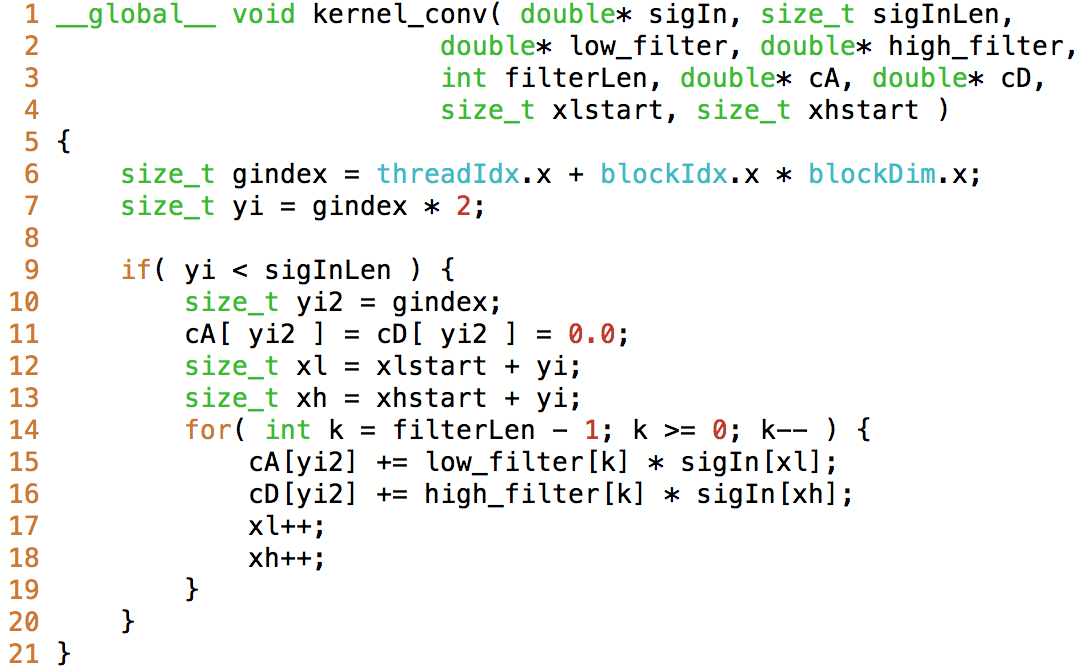
\includegraphics[width=0.9\textwidth]{conv.png}
    \caption{CUDA kernel for performing convolution on the input signal
             with the low-pass and high0pass wavelet kernels.}
    \label{fig:conv1}
\end{figure}

Note that the \verb|__global__| syntax indicates that this is a CUDA kernel
to be executed on the GPU.
%
Each thread finds out the index of itself in line~6, and checks if it is
within the data range before proceeding (line~9).


The invocation of a CUDA kernel also differs from calling a C function.
%
More specifically, we need to pass two pieces of information to the GPU:
how many thread in a block, and how many blocks in a grid.
%
These two pieces of information are specified using a triple, indicating
the three dimension of a thread block and a grid.
%
The syntax to invoke a CUDA kernel is as follows:

\bigskip
\noindent \verb|kernel_conv<<< (nBlock, 1, 1), (nThread_Per_Block, 1, 1) >>> ();|
\bigskip

The last mandatory routine to use CUDA kernels is to manage the memory
on the GPU card, including allocating memory, copy data back and forth from
the system RAM, and free the allocated memory on GPU.
%
The following piece of code illustrates the routine of allocating a chunk of 
memory on GPU, copying data from RAM to GPU, copy the result from GPU to RAM,
and free the allocated memory.

\bigskip
\noindent \verb| double *d_in; | \\
\verb| int d_size = sizeof( double ); | \\
\verb| cudaMalloc( (void**) &d_in, inLen * d_size ); |    \\
\verb| cudaMemcpy( d_in, in, inLen * d_size, cudaMemcpyHostToDevice ); |\\
\verb| cudaMemcpy( out, d_out, outLen * d_size, cudaMemcpyHostToDevice ); |\\
\verb| cudaFree( d_in ); |
\bigskip


\subsection{Shared Memory}
\label{sec:sharedM}
%
Shared memory lies in the GPU memory hierarchy between the global memory,
which can be accessed by all CUDA cores, and the registers, which can only 
be accessed by the single CUDA cores.
%
Instead, shared memory is associated with each single CUDA multiprocessor, 
and thus being accessable by all the CUDA cores in that multiprocessor.
%
Because shared memory is significantly faster than global memory,
a program can benefit from storing repeatedly accessing data in 
shared memory, instead of global memory.
%
In my case, the wavelet filters are retrieved by each thread to perform
convolution, and shoould be put in the shared memory to increase the performance.
%
The following piece of code shows that we declear a chunck of shared memory to hold
the wavelet filter, and each thread fills one data element.

\bigskip
\noindent \verb| __shared__ double s_low_filter[ 9 ]; | \\
\verb| __shared__ double s_high_filter[ 9 ]; |\\
\verb| if( threadIdx.x < 9 ) { |\\
\verb|     s_low_filter[ threadIdx.x ] = low_filter[ threadIdx.x ]; |\\
\verb|     s_high_filter[ threadIdx.x ] = high_filter[ threadIdx.x ]; |\\
\verb| } |\\
\verb| __syncthreads();|
\bigskip

Note that since all threads are executed concurrently, there is a chance that
some threads try to read from the shared memory, before it is initialized.
%
To prevent this from happening, we add a \verb|__syncthreads()| line after
initializing the shared memory.


\section{Performance Study}
\label{sec:performance}
%
To study the performance of DWT using CUDA, as well as different parameters
of CUDA, I experimented on three perspectives:
%
\begin{enumerate}
\item How much speedup compared to a serial implementation?
\item How much the employment of shared memory improve the  performance?
\item How does the thread-per-block parameter affect the performance?
\end{enumerate}


\subsection{Speedup Tests}
\label{sec:speedup}
%
To test the speedups that GPU brings to DWT, I tested my CUDA implementation against
the serial implementation on a CPU.
%
The GPU card that I'm testing on is an Nvidia Tesla K40 GPU with 2,880 CUDA cores
and 12GB memory.
%
The CPU that I'm testing on is an Intel Xeon E5-2680 v2 Ivy Bridge processor at 2.8GHz.
%
The serial code was also compiled using the Intel compiler and the \verb|-O3| optimization
option.

The test data set was a float array of 512 million points. 
%
I tested on this array using part or the whole length of it, 
eight differences ranging from 64 million to 512 million, to see what the speedup
is at each of the problem sizes. 
%
Figure~\ref{fig:speedup} summarizes the test results, with 
the blue showing CUDA execution time,
the red line showing serial execution time, 
and the orange line showing the achieved speedups.
%
Note that the right vertical axis is for the speedups.

\begin{figure}
    \centering
    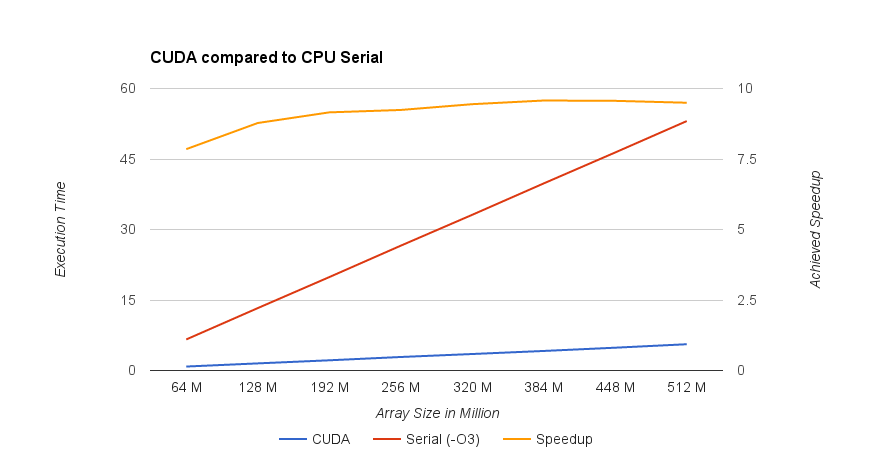
\includegraphics[width=1\textwidth]{speedup.png}
    \caption{Execution time of DWT on different problem sizes (in seconds),
             and the corresponding speedups.
             Notice that the speedup reads are on the right vertical axis.}
    \label{fig:speedup}
\end{figure}

The results show that GPU achieves a consistant 9x speedup when the problem size
is big enough, i.e., 256 million.
%
Even at smaller problem sizes, the speedups are also above 7.5x, which are 
also encouraging.
%
The overall performance of GPU meets my expectation.


\subsection{Threads Per Block and Shared Memory Study}
%
Threads per block is an important parameter in launching a CUDA kernel.
%
It should always be a multiplication of 32, bacaues CUDA always groups
threads into a ``warp" of size 32 to perform tasks.
%
The optimal number is determined by both the hardware capability, e.g., 
how many CUDA cores are there in a CUDA multiprocessor, as well as the 
specific problem to tackle. 
%
Empirically, the optimal value is somewhere between 128 and 512.

Shared memory speeds up data retrieving (see Section~\ref{sec:sharedM}),
so it is expected to help improve the overall performance.

My test varied the thread-per-block parameter from 32 to 256 with eight
values in total.
%
With each thread-per-block value, I tested the performance with or without 
the use of shared memory.
%
These configurations result in sixteen tests in total. 
%
I used the 512 million data size for this test.
%
Figure~\ref{fig:3} presents the execution times with different
configurations in seconds.


\begin{figure}
    \centering
    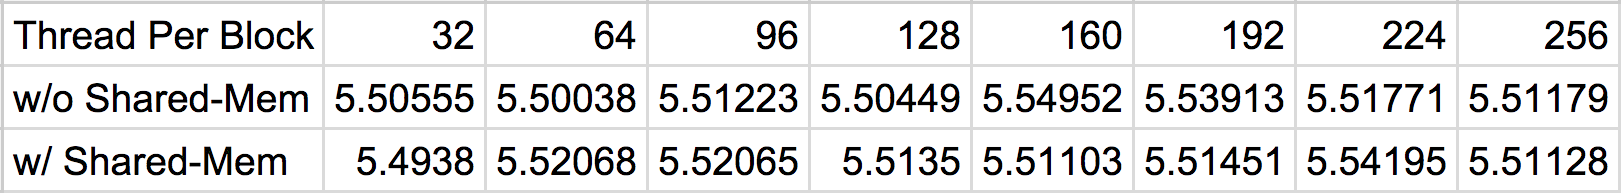
\includegraphics[width=1\textwidth]{3.png}
    \caption{Execution time of DWT with different threads-per-block parameter,
             and the configuration with or without shared memory.}
    \label{fig:3}
\end{figure}


Surprisingly, the execution times using various configurations are quite
consistant: they are all at around 5.5 seconds.
%
Even the use of shared memory did not affect the performance.

One hypothesis that could possibly explain why the use of shared memory
did not improve performance, was that the amount of data I manually
put in the shared memory is too small (18 doubles in my case).
%
Because these wavelet filters are retrieved once and once again,
it is possible that they are kept in the shared memory.
%
This hypothesis needs more evidence to support.

I am not able to explain why the thread per block parameter does not
affect the performance at all.


\section{Conclusions}
%
We demonstrated in this project that GPU (especially Nvidia GPUs with CUDA)
is effective in speeding up programs 
using a stencil parallel processing pattern.
%
The speedups exhibit good scalability, which means GPU with CUDA could potentially 
be used in problems with much larger scales.


At the same time, CUDA programming differs from traditional C++ programming
in that it requires more tuning to achieve the best performance.
%
This indicates a steeper learning curve of employing CUDA as a productive tool.

 

%\section{Expected Results}
%
%The expected result of this project is a stable and practically useful 
%implementation of the DWT on many-core architectures.
%%
%Along this process, I will gain more understanding on parallel
%computing, as well as the wavelet transform itself.
%
%The ultimate goal is to get myself ready for algorithm designing and 
%programming for the many-core architectures in the future.



\bibliographystyle{plain}
\bibliography{main}
\end{document}
